\section{Demo-frontend}
\label{sec:demo-frontend}

VideoAPI er et mellomvare-API uten eget brukergrensesnitt. For å kunne
demonstrere systemet for HDO og verifisere at endepunktene fungerer
ende-til-ende ble det utviklet en enkel referanseklient i et separat prosjekt.
Frontenden dekker hele den forventede arbeidsflyten --- innlogging,
romadministrasjon, sending og visning --- og er bevisst holdt enkel uten
forretningslogikk utover det API-et selv tilbyr. Løsningen er utviklet som en demonstrasjonsleveranse og skal ikke betraktes som en produktleveranse.

\subsection{Teknologivalg}
\label{subsec:demo-tech}

Tabell~\ref{tab:frontend-tech} oppsummerer de sentrale teknologiene.
React med TypeScript ble valgt på bakgrunn av tidligere gruppeerfaring, og
typesystemet gjør det enkelt å speile API-ets responsformer direkte i
klientkoden. Vite gir rask hot reload under utvikling og produserer et statisk
bundle som kan serveres uten en aktiv Node-prosess. For WebRTC-strømmingen
brukes AntMedias offisielle adapter, som håndterer \gls{ice}-forhandling og
signalering slik at koden kan konsentrere seg om brukerflyt fremfor
lavnivå-detaljer.

\begin{table}[H]
\centering
\caption{Sentrale teknologier i demo-frontenden.}
\label{tab:frontend-tech}
\begin{tabular}{l l}
\toprule
\textbf{Lag} & \textbf{Teknologi} \\
\midrule
UI-rammeverk        & React 19 + TypeScript \\
Byggeverktøy        & Vite 7 \\
Styling             & Tailwind CSS 4 \\
Ruting              & React Router 7 \\
WebRTC-klient       & \texttt{@antmedia/webrtc\_adaptor} 2.16 \\
Produksjonsserver   & nginx (Alpine) \\
Containerisering    & Docker + Docker Compose \\
\bottomrule
\end{tabular}
\end{table}

\subsection{Applikasjonsstruktur og autentisering}
\label{subsec:demo-struktur}

Applikasjonen har fem sider: \texttt{Login}, \texttt{Dashboard}, \texttt{Room},
\texttt{Broadcast} og \texttt{Watch}. Kildekoden er organisert etter teknisk
rolle med mapper for sider, komponenter, API-kall, hooks og typedefinisjoner.
Typedefinisjonene speiler API-ets \gls{dto}-er direkte, slik at endringer i
API-kontrakten typisk gir kompilatorfeil på klientsiden.

Innlogging skjer ved at frontenden sender en forespørsel mot \texttt{/auth/token}-endepunktet med \texttt{clientId} og \texttt{clientSecret}, som vist i figur~\ref{fig:frontend-login-dashboard}a. Tokenet lagres i \texttt{sessionStorage} og utløper etter fire minutter, noe kortere enn Keycloaks levetid. Brukeren sendes deretter automatisk tilbake til \texttt{Login} (innloggingssiden) når sesjonen utløper. Alle API-kall går gjennom en felles hjelper som setter \texttt{Authorization}-headeren og håndterer \texttt{401 Unauthorized}-svar sentralt. Etter innlogging vises \texttt{Dashboard} (jf. figur~\ref{fig:frontend-login-dashboard}b), som henter tilgjengelige providers fra \texttt{/health/ready} og lister opp eksisterende rom.

% \begin{figure}[H]
%     \centering
%     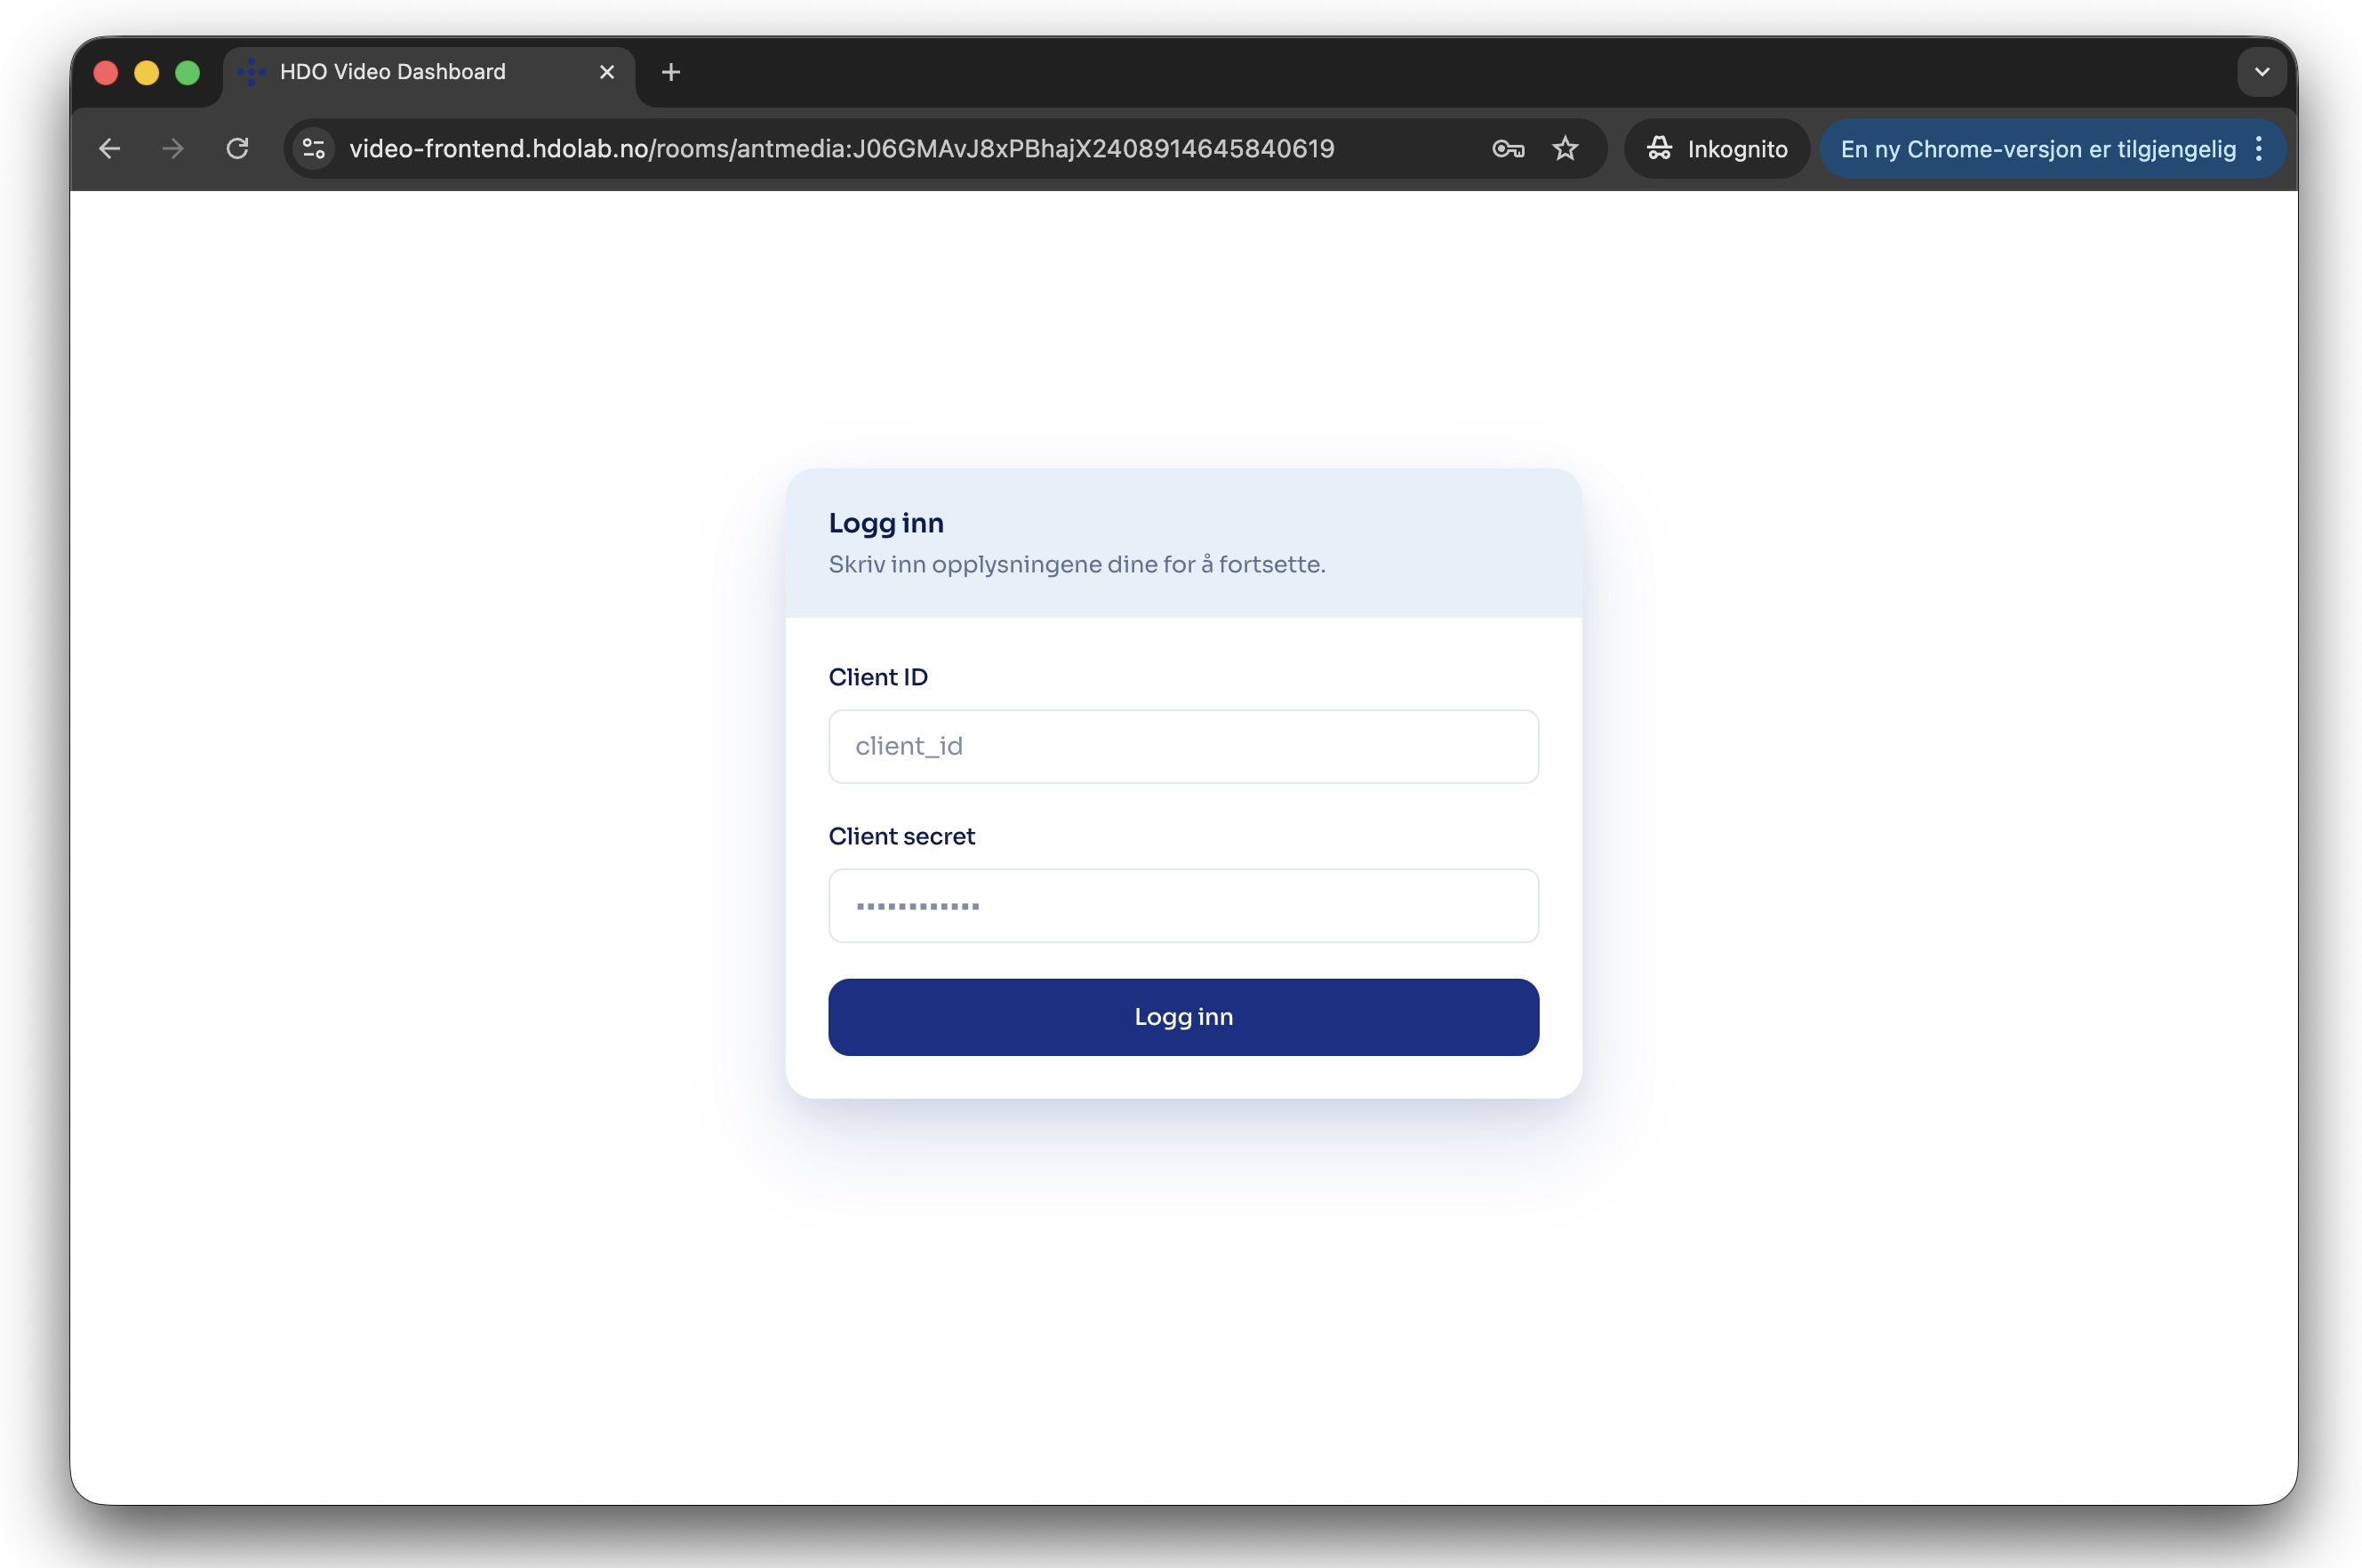
\includegraphics[width=0.9\linewidth]{figures/hdo-login.jpg}
%     \caption{\texttt{Login} -- innloggingsside.}
%     \label{fig:frontend-login}
% \end{figure}

% \begin{figure}[H]
%     \centering
%     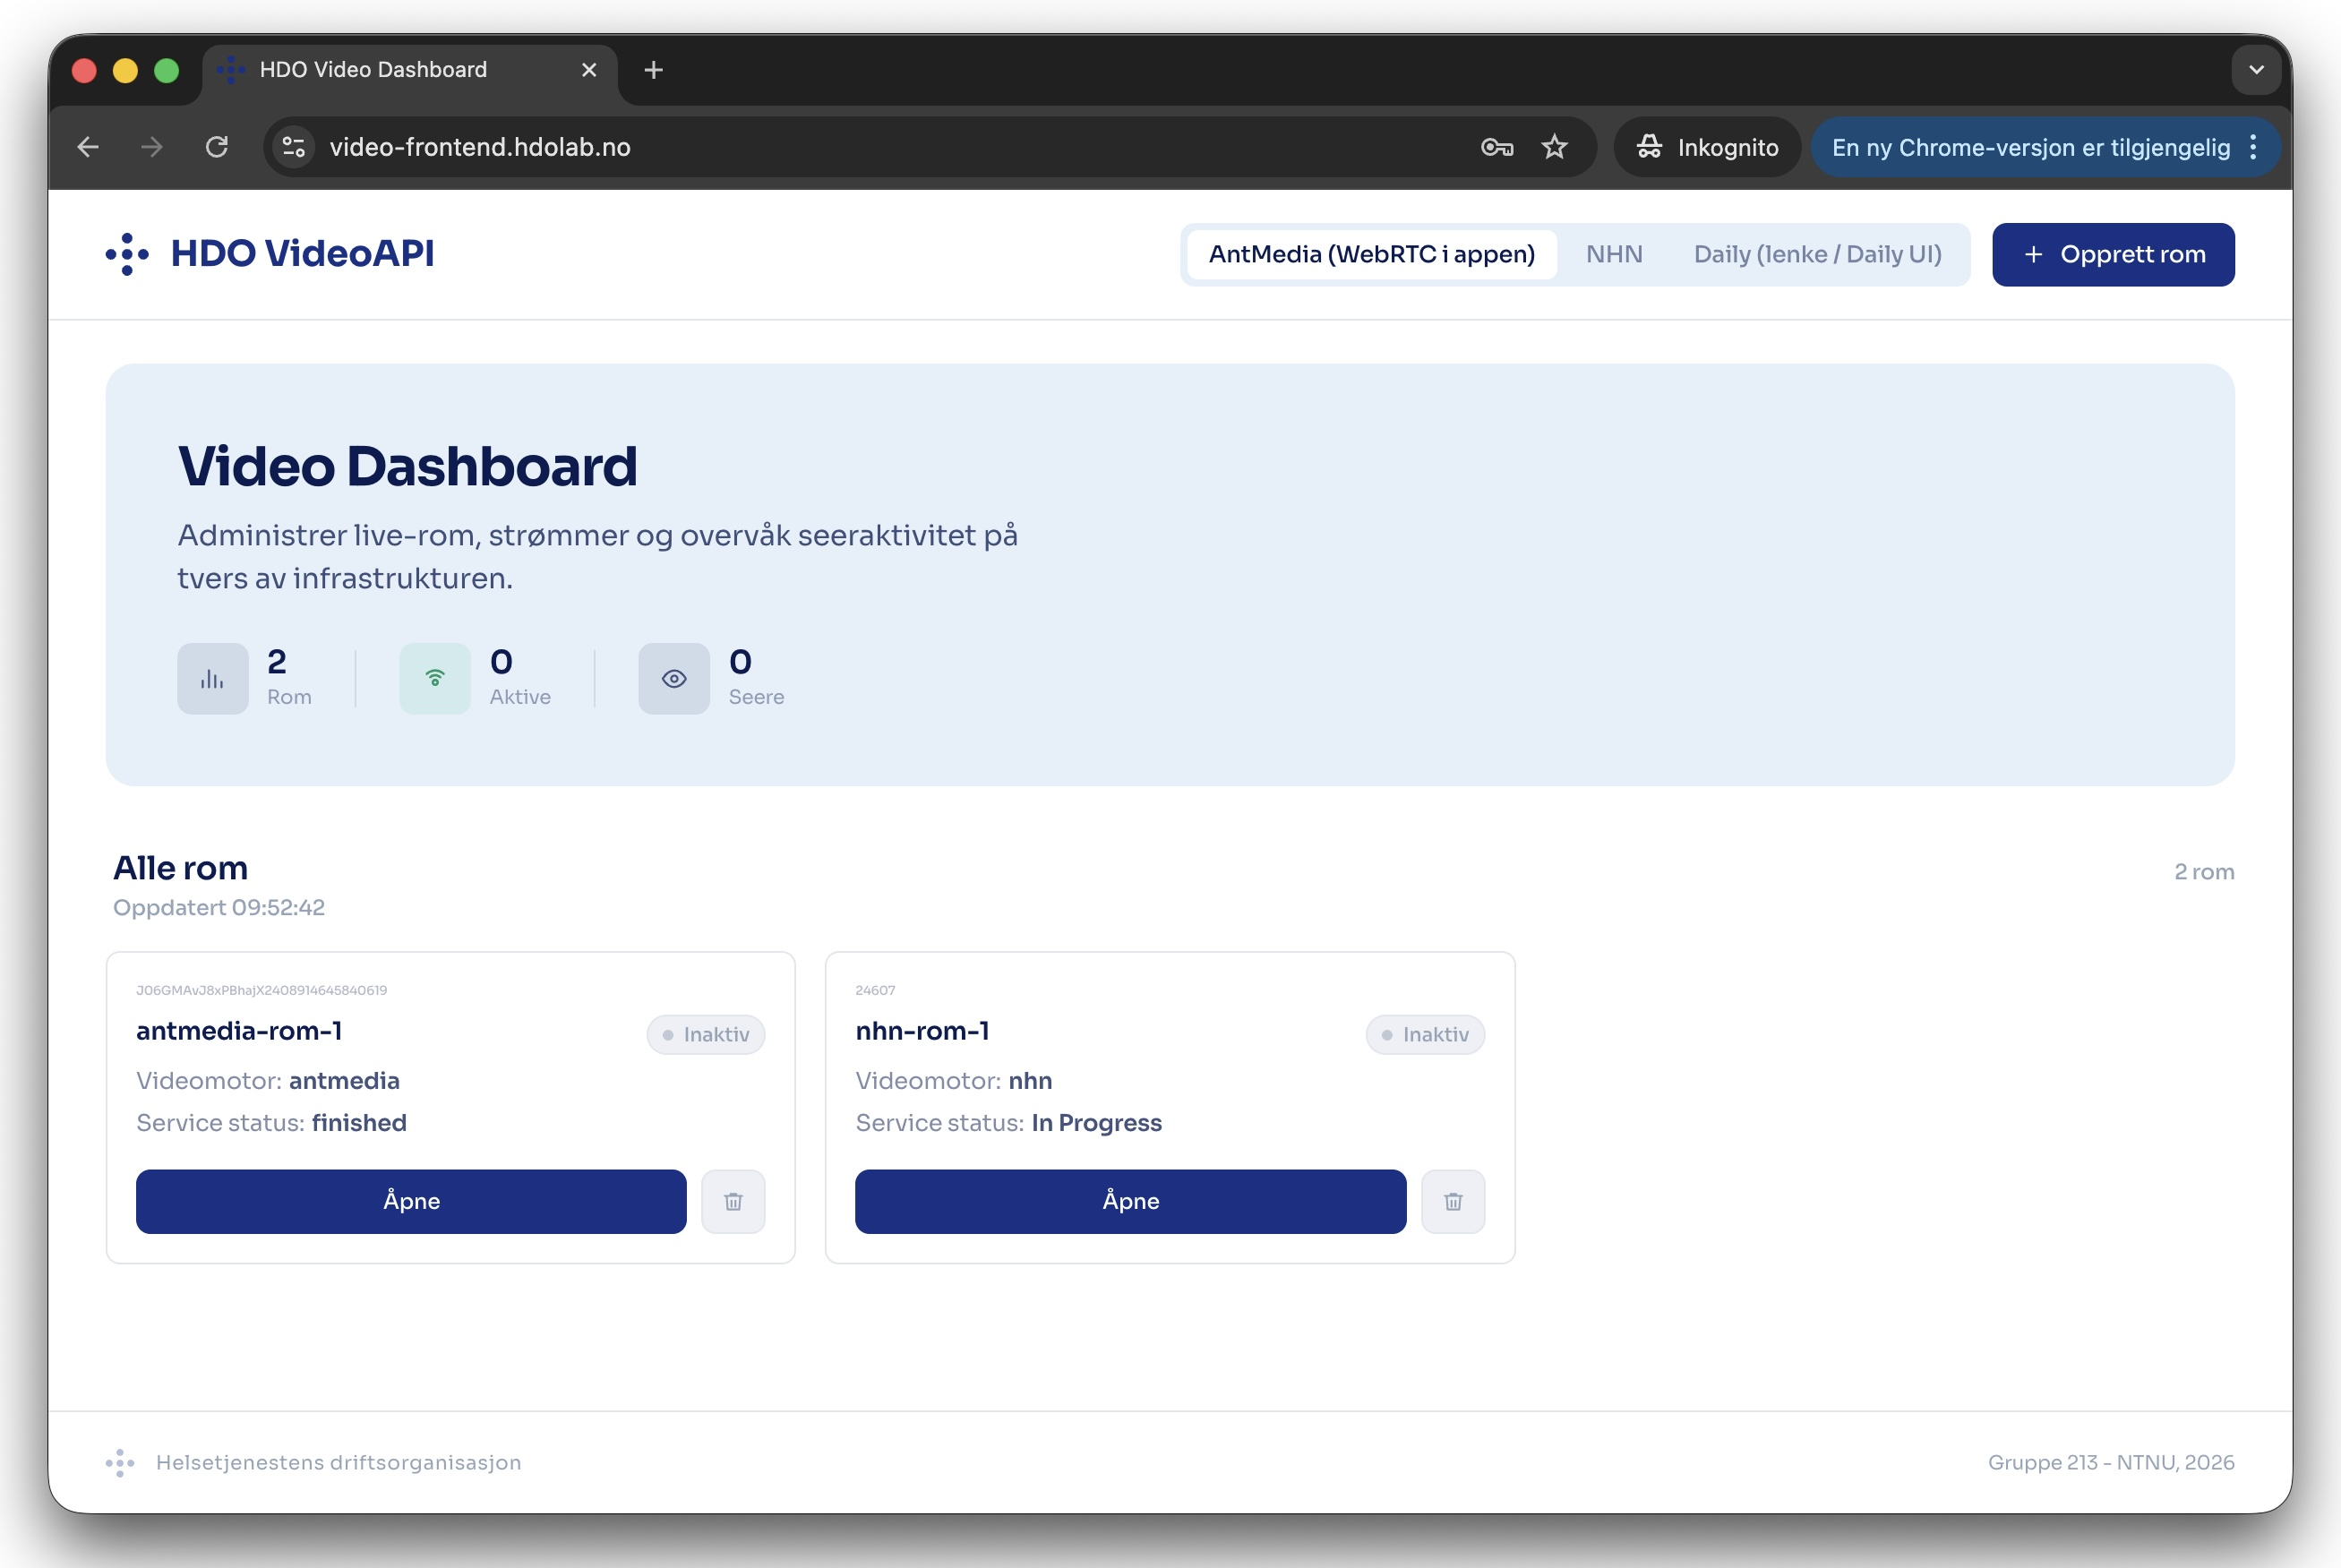
\includegraphics[width=0.9\linewidth]{figures/hdo-dashboard.jpg}
%     \caption{\texttt{Dashboard} -- oversiktsside.}
%     \label{fig:frontend-dashboard}
% \end{figure}

\newpage
\begin{figure}[H]
  \centering
  \begin{minipage}[t]{1\textwidth}
    \centering
    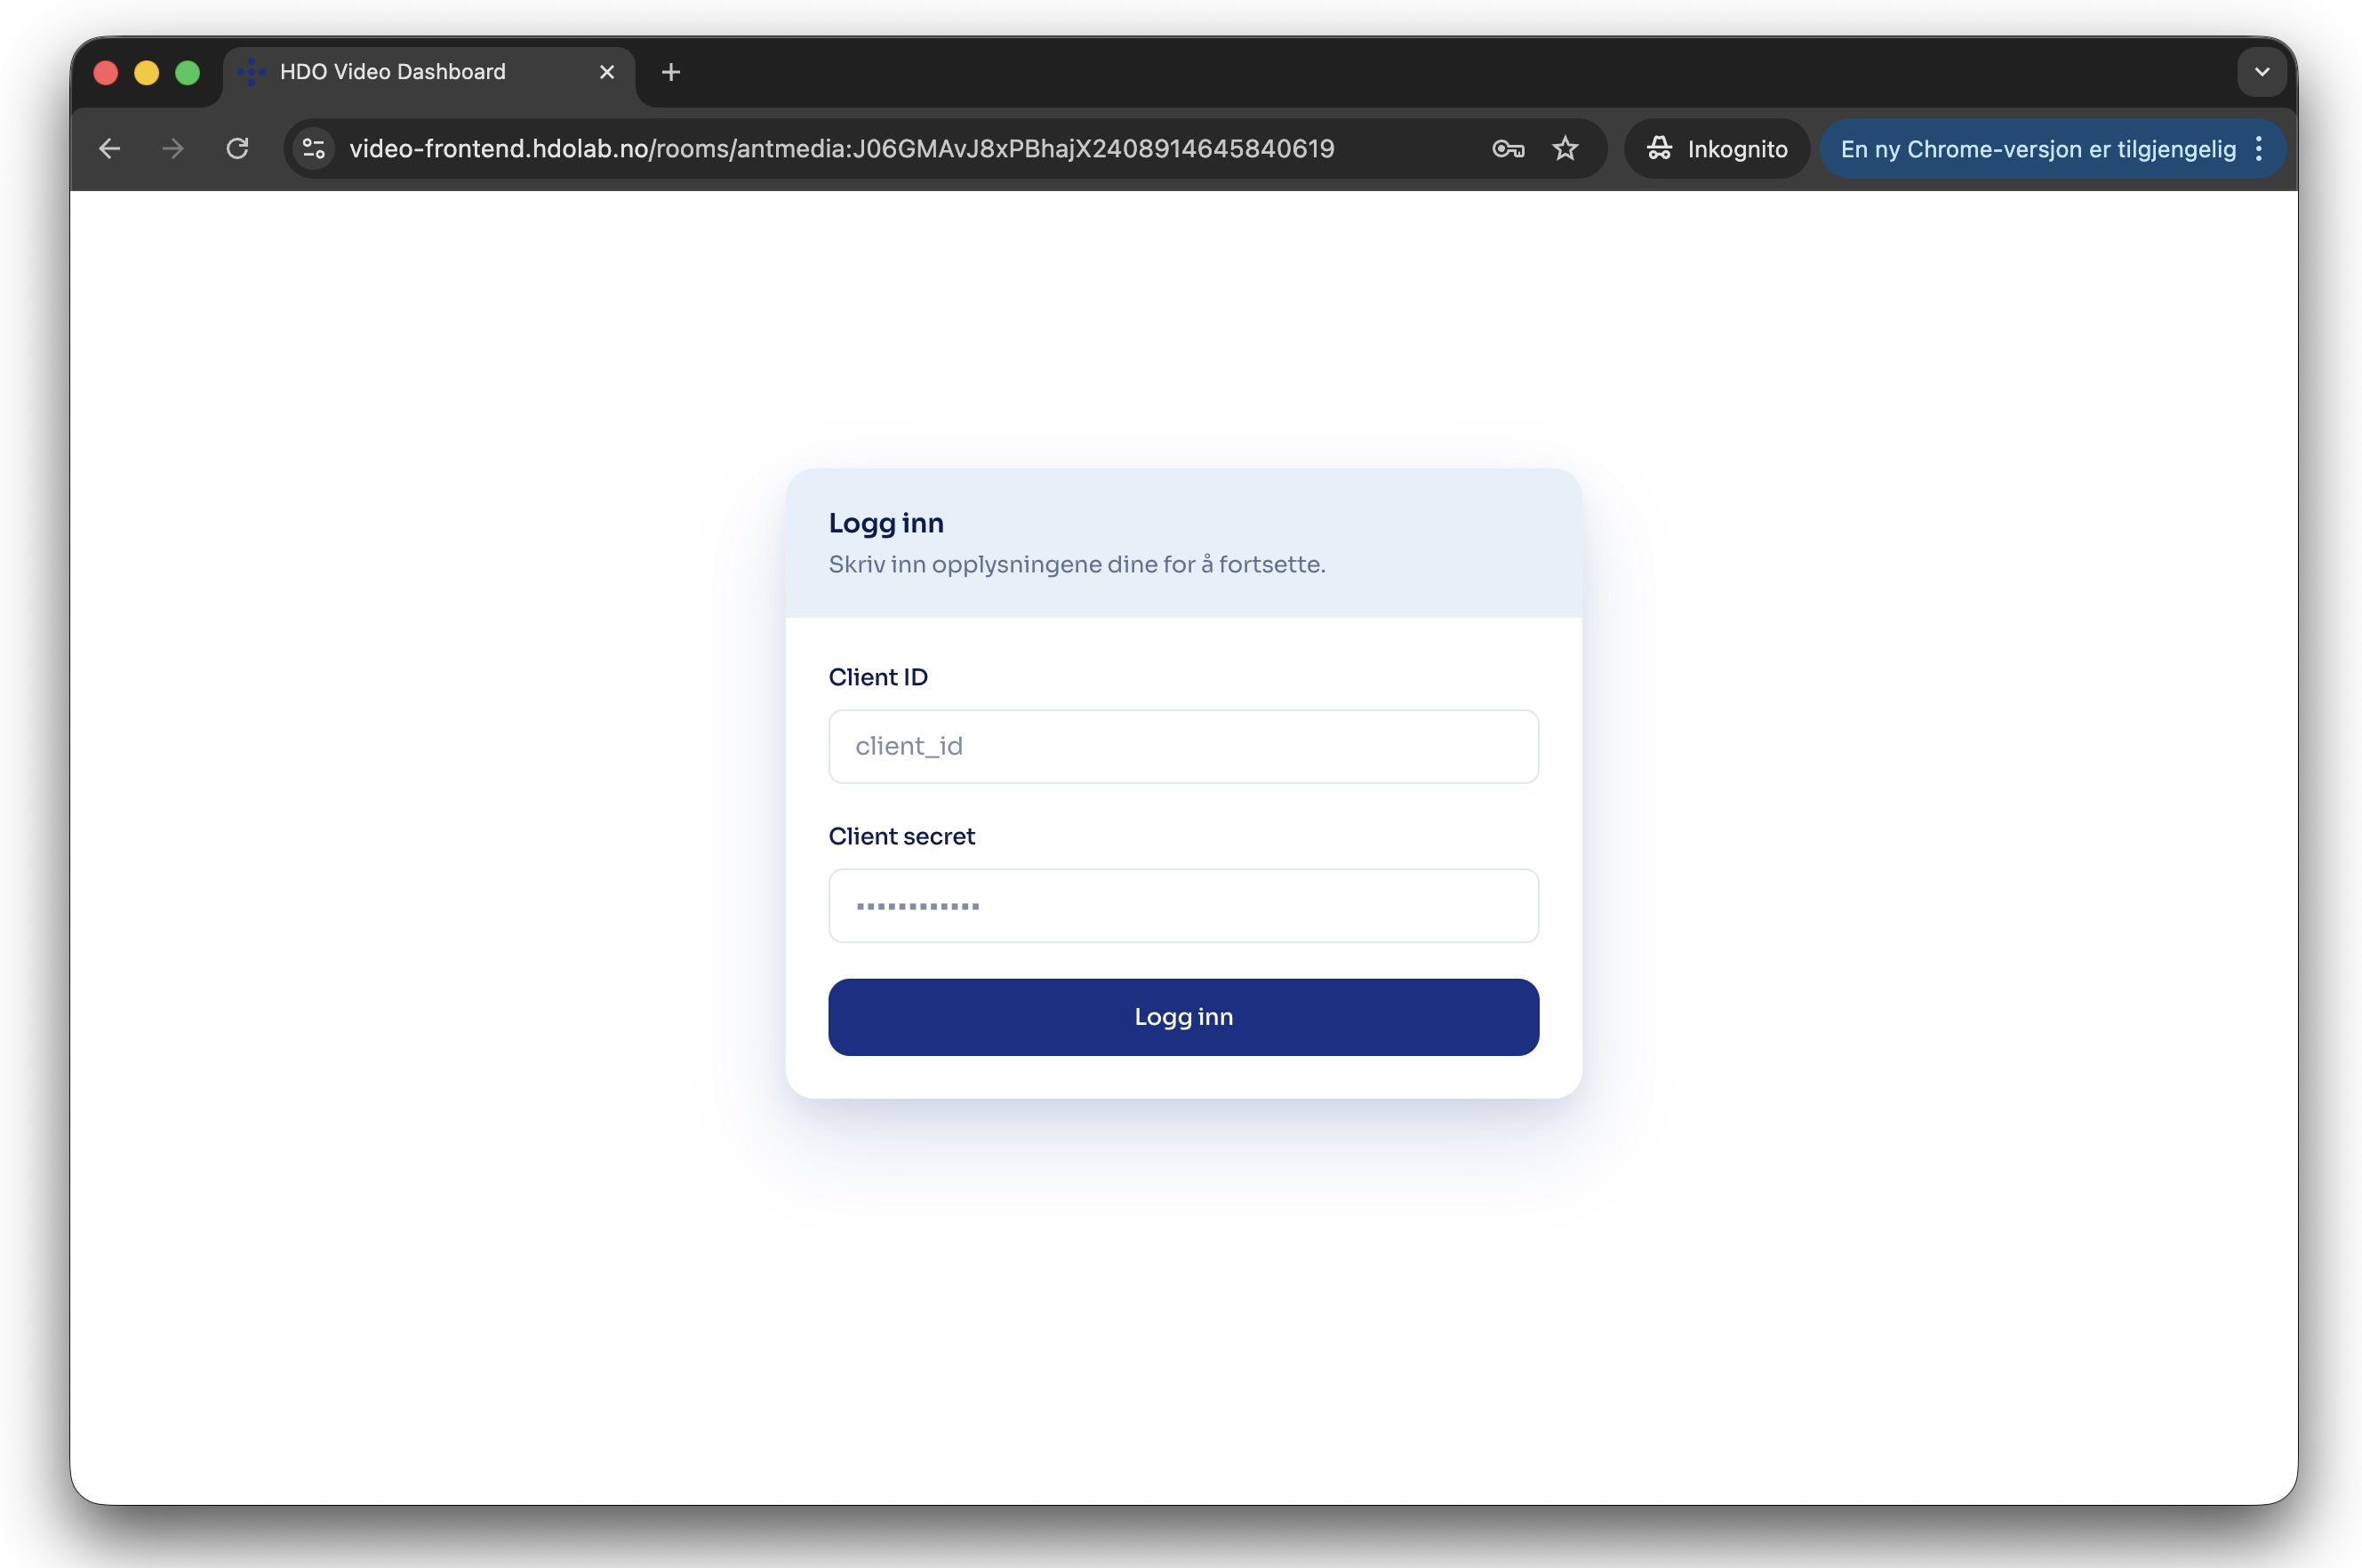
\includegraphics[width=\linewidth]{figures/hdo-login.jpg}
    \caption*{(a) \texttt{Login} -- Innloggingssiden}
  \end{minipage}
  \hfill
  \begin{minipage}[t]{1\textwidth}
    \centering
    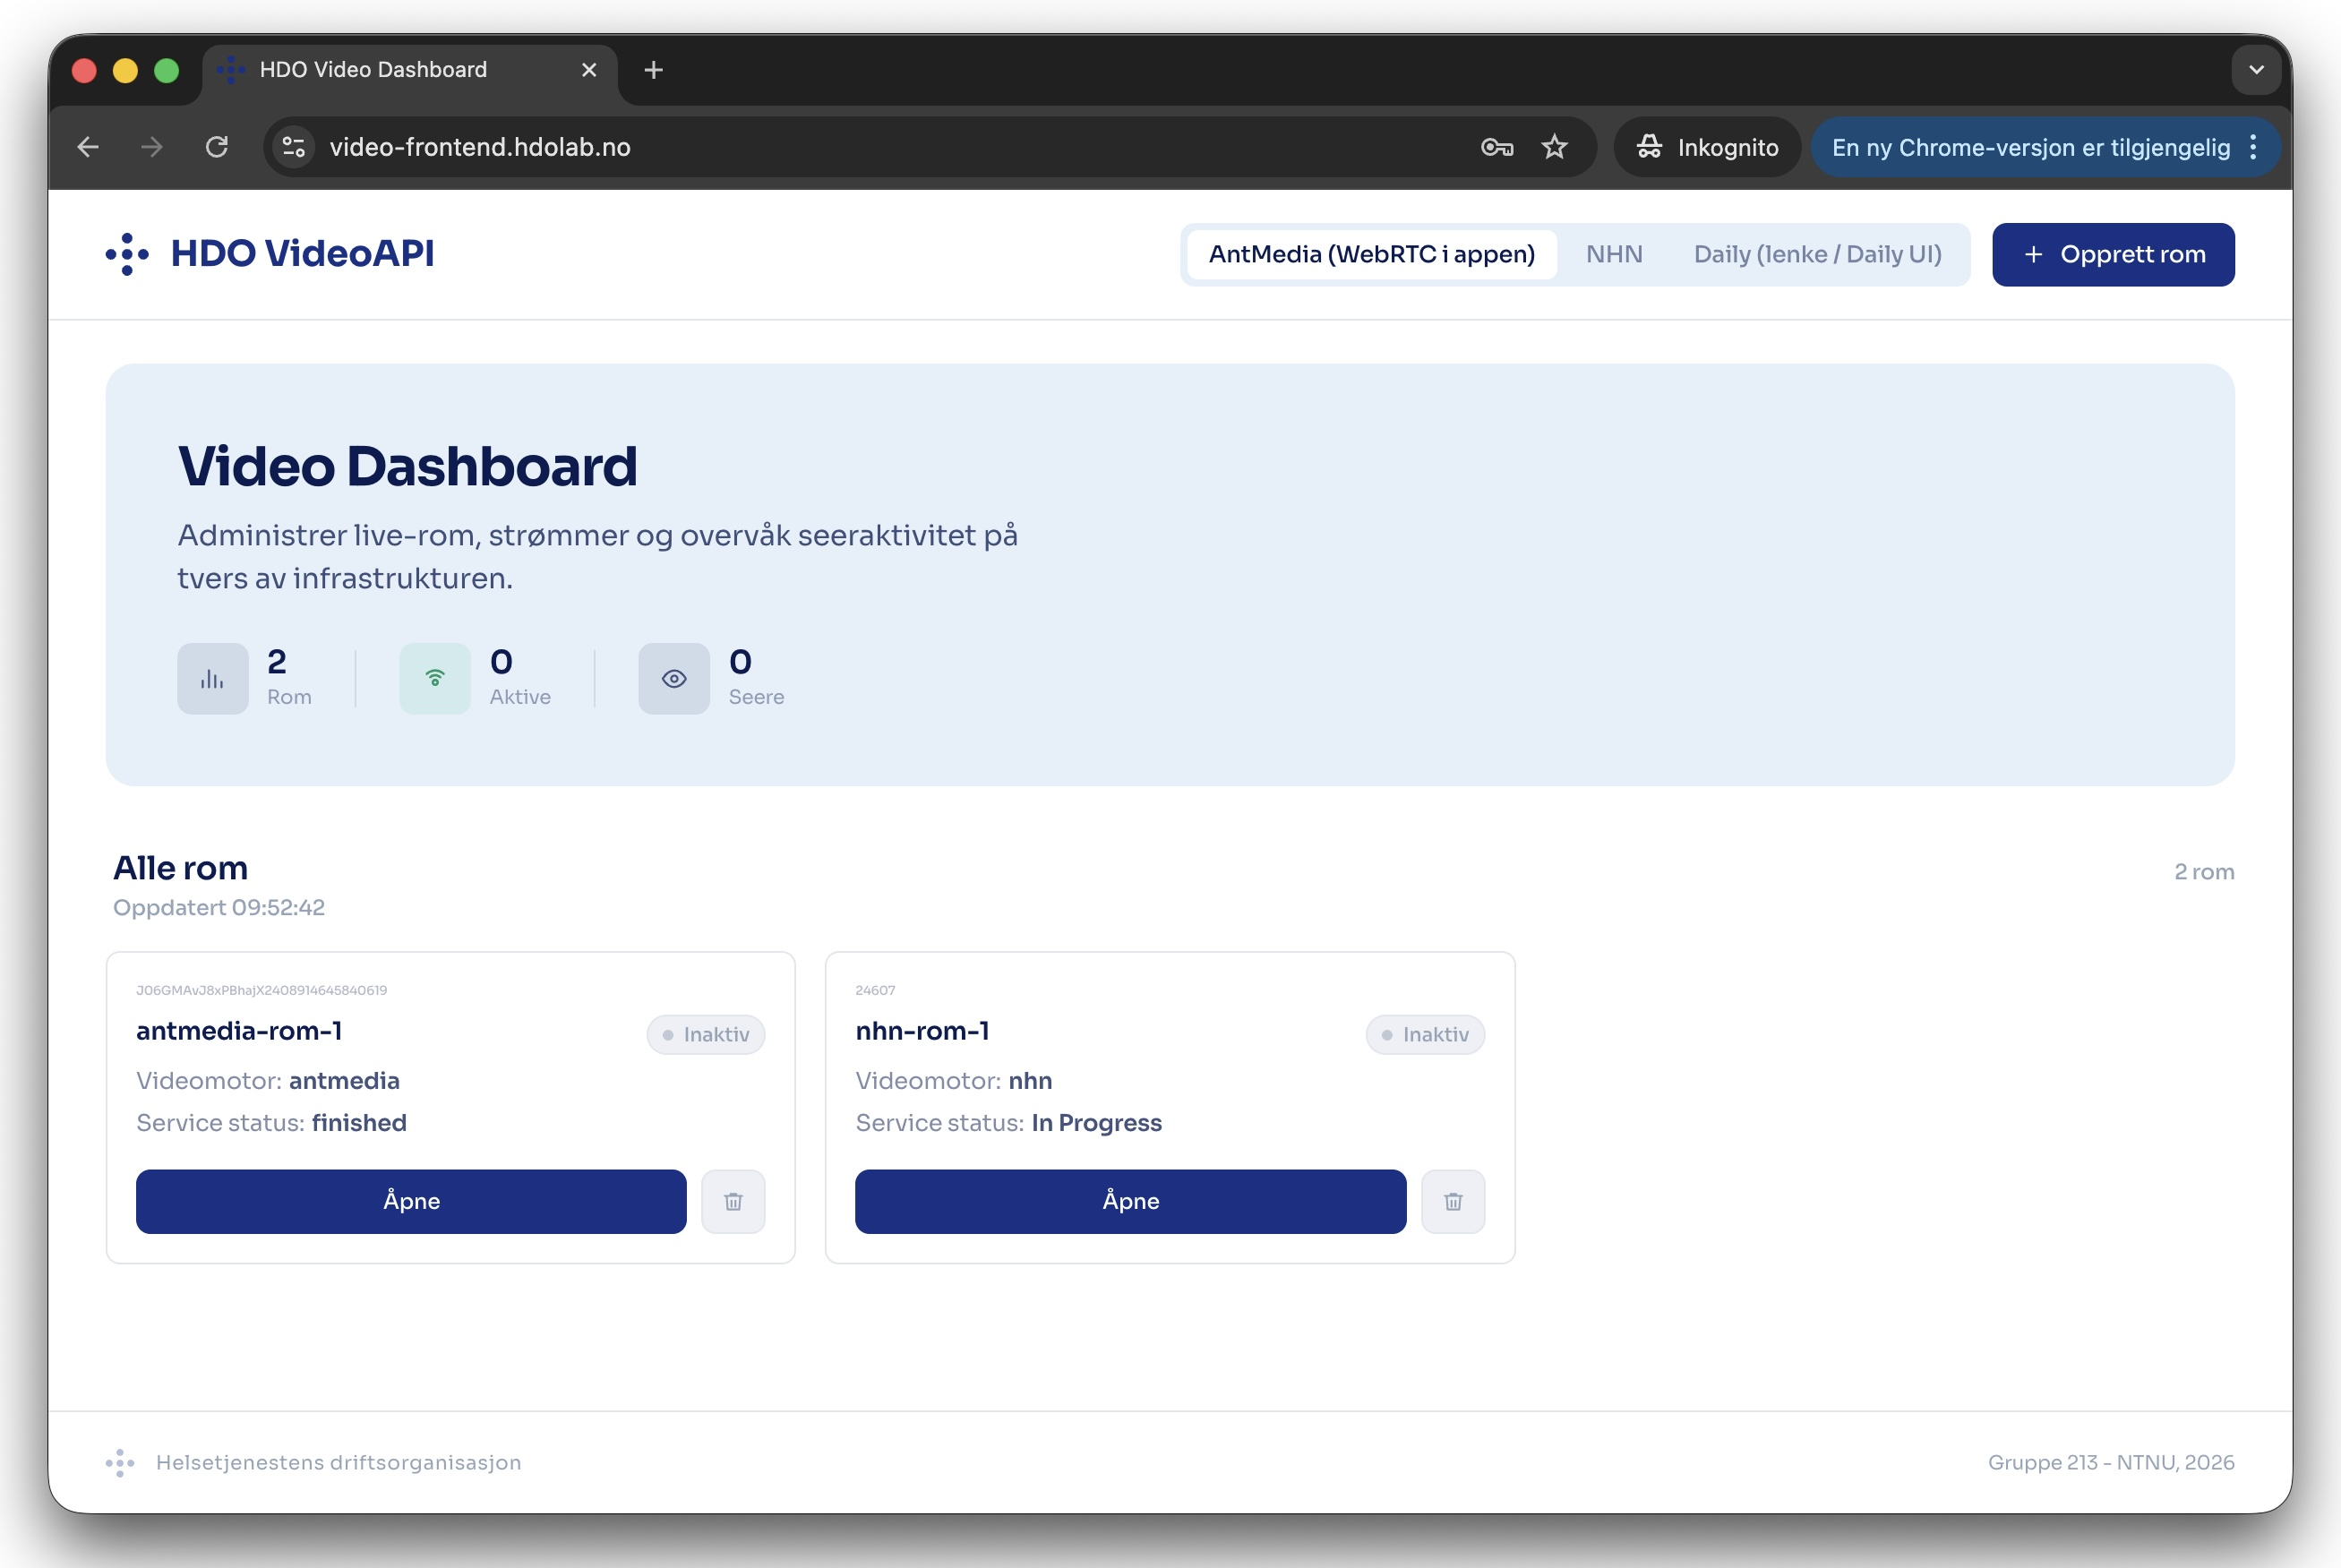
\includegraphics[width=\linewidth]{figures/hdo-dashboard.jpg}
    \caption*{(b) \texttt{Dashboard} -- oversiktsside}
  \end{minipage}
  \caption{Demo-frontenden: innlogging og oversiktsside.}
  \label{fig:frontend-login-dashboard}
\end{figure}

% Innlogging skjer mot \texttt{/auth/token} med \texttt{clientId} og \texttt{clientSecret}. Tokenet lagres i \texttt{sessionStorage} og utløper etter fire minutter, noe kortere enn Keycloaks levetid. Brukeren sendes deretter automatisk tilbake til innloggingssiden når sesjonen utløper. Alle API-kall går gjennom en felles hjelper som setter \texttt{Authorization}-headeren og håndterer \texttt{401 Unauthorized}-svar sentralt.

% Sender- og mottakersidene (\texttt{Broadcast} og \texttt{Watch}) bruker en
% annen mekanisme: frontenden kaller
% \texttt{POST /api/rooms/\{provider\}:\{id\}/webrtc-link} og får tilbake en
% korttidsgyldig stream-token som legges som \texttt{?token=}-parameter i
% delelenken. Tokenen verifiseres direkte av AntMedia ved WebRTC-tilkoblingen,
% slik at deltakere kan sende eller se uten egen Keycloak-konto.

\subsection{Ende-til-ende-flyt: rom og videostrøm}
\label{subsec:demo-flyt}
For å illustrere den fulle arbeidsflyten tas rommet \texttt{antmedia-rom-1}
som eksempel. Fra \texttt{Dashboard} velger brukeren rommet og kommer til
\texttt{Room}-siden (jf. figur~\ref{fig:frontend-room}), som viser rommets status og gir
tilgang til \texttt{Broadcast}- og \texttt{Watch}-lenkene.

\begin{figure}[H]
  \centering
  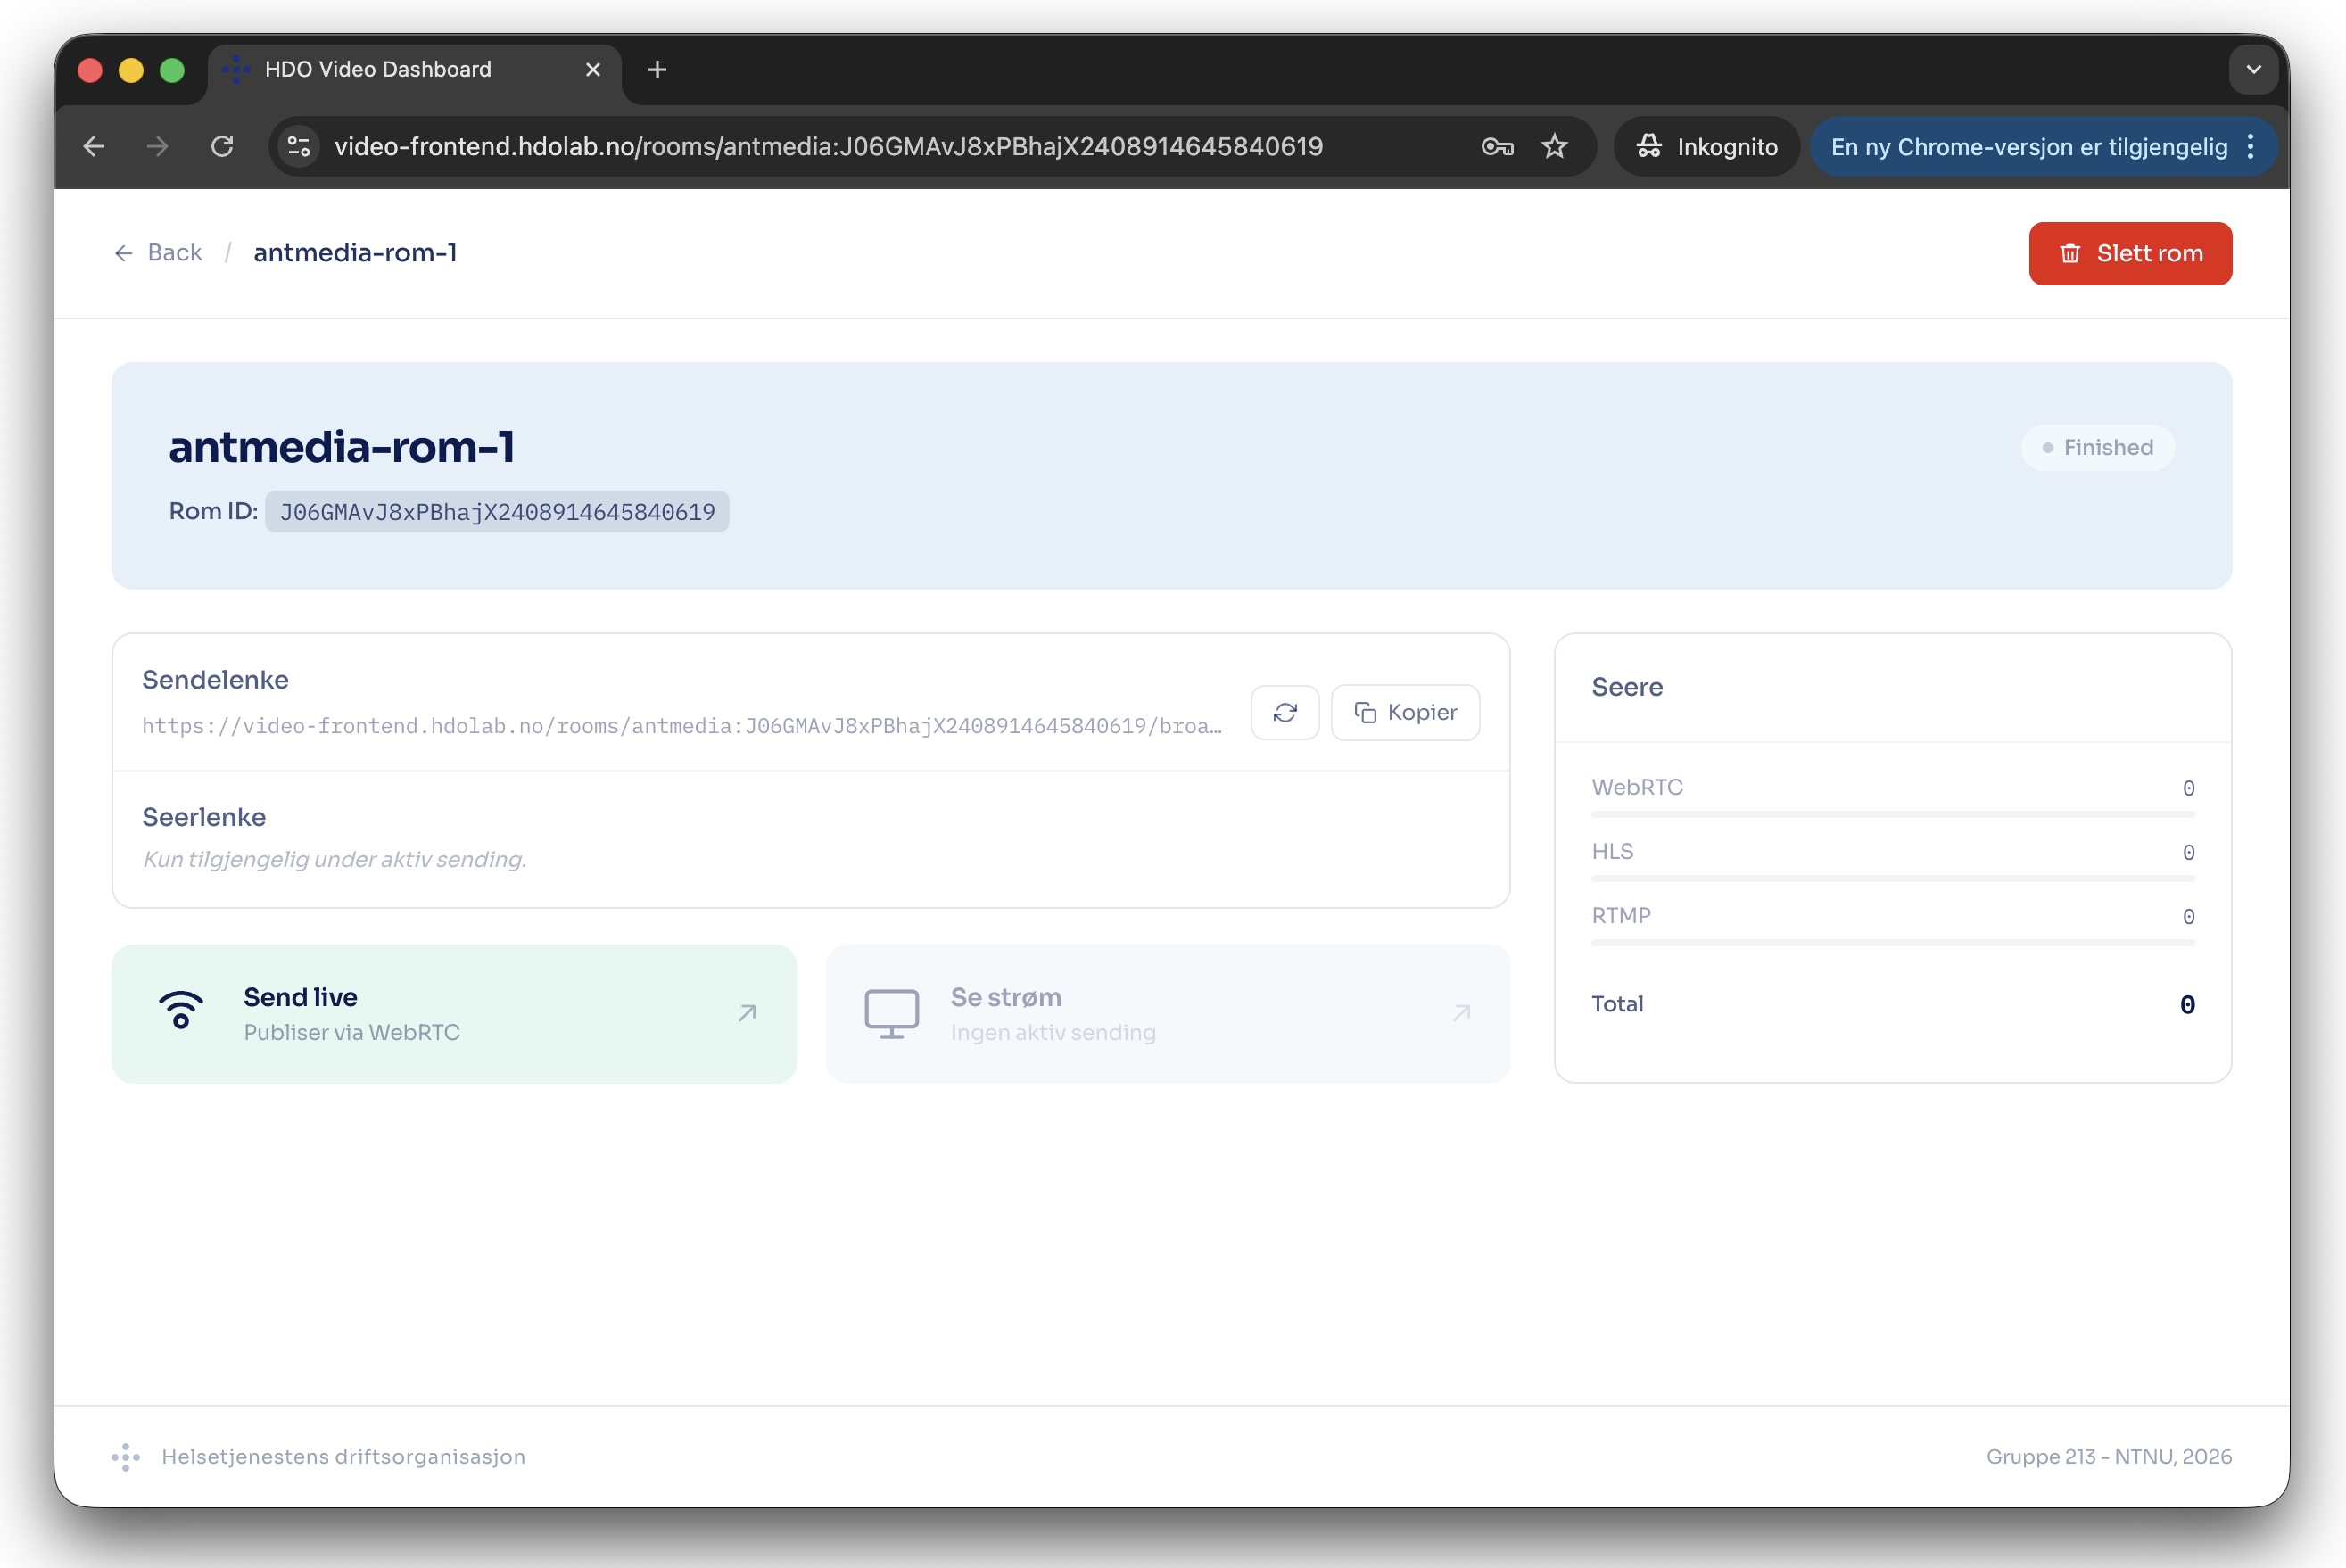
\includegraphics[width=1\textwidth]{figures/hdo-rom.jpg}
  \caption{\texttt{Room}-siden for \texttt{antmedia-rom-1} med strømalternativer.}
  \label{fig:frontend-room}
\end{figure}

% Når en deltaker trykker på Broadcast- eller Watch-knappen, kaller frontenden
% \texttt{POST /api/rooms/\{provider\}:\{id\}/webrtc-link} og får tilbake en
% korttidsgyldig stream-token. Tokenen legges som \texttt{?token=}-parameter i
% lenken og verifiseres direkte av AntMedia ved WebRTC-tilkoblingen, slik at
% verken avsender eller mottaker trenger en Keycloak-konto for å delta.

Når en bruker trykker på \texttt{Broadcast}- eller \texttt{Watch}-knappen, kaller frontenden
\url{POST /api/rooms/{provider}:{id}/webrtc-link} og får tilbake en
korttidsgyldig stream-token. Tokenen legges som \texttt{?token=}-parameter i
lenken og verifiseres direkte av AntMedia ved WebRTC-tilkoblingen.

Herfra kan én deltaker åpne \texttt{Broadcast}-lenken --- i dette tilfellet fra en
mobiltelefon --- og starte WebRTC-publiseringen.
Figur~\ref{fig:frontend-broadcast-watch}a viser kamerabildet slik det fremstår
på avsenderenheten under en aktiv strøm. Samtidig kan en annen deltaker åpne
\texttt{Watch}-lenken fra en annen enhet, for eksempel en PC, og se strømmen direkte i
nettleseren (figur~\ref{fig:frontend-broadcast-watch}b). Tokenene er generert og verifiseres av AntMedia; verken avsender eller mottaker trenger
en Keycloak-konto for å delta.

\begin{figure}[H]
  \centering
  \begin{minipage}[c]{0.26\textwidth}
    \centering
    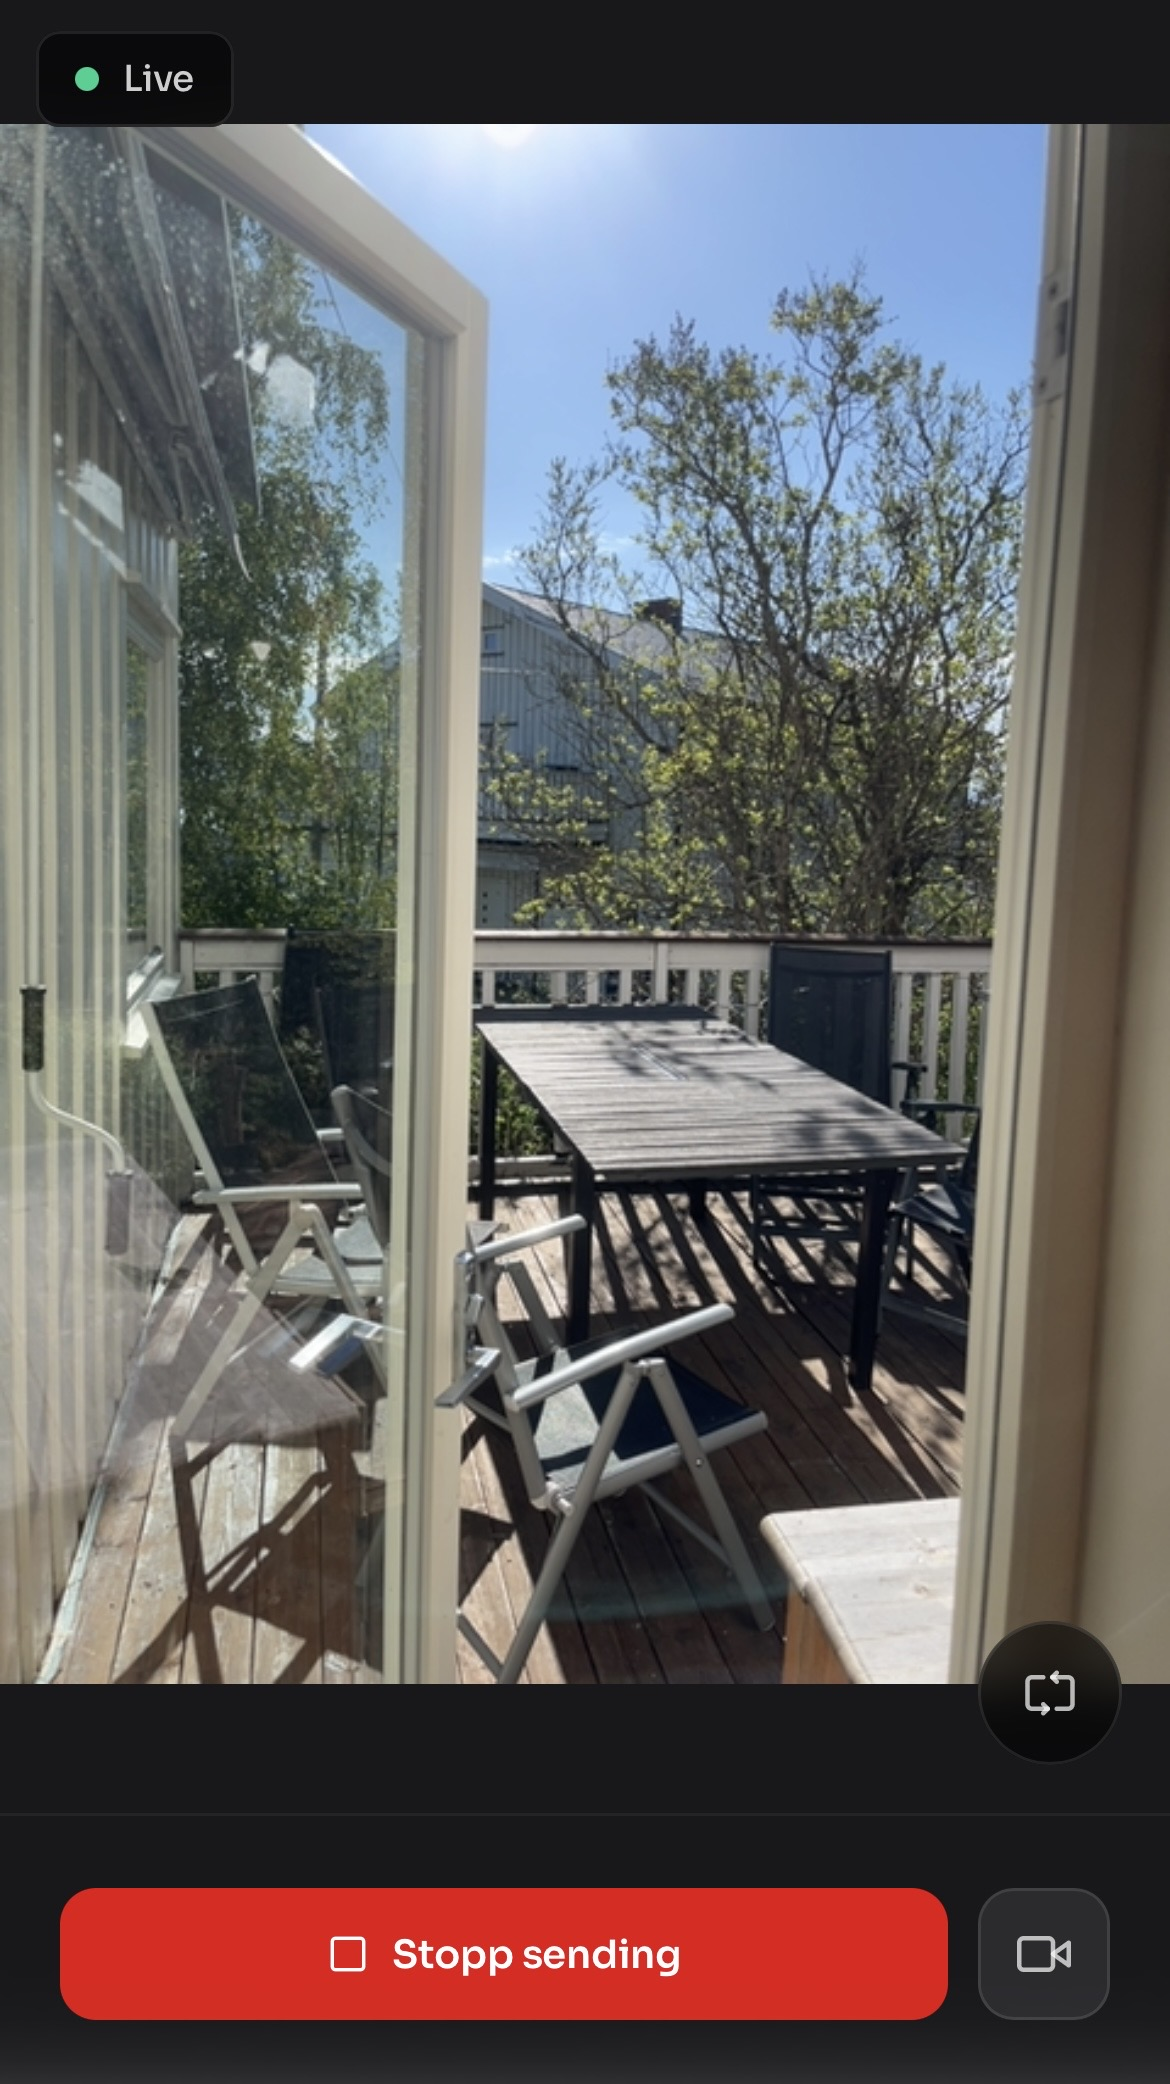
\includegraphics[width=\linewidth]{figures/hdo-broadcast-tlf.jpg}
    \caption*{(a) \texttt{Broadcast}}
  \end{minipage}
  \hfill
  \begin{minipage}[c]{0.71\textwidth}
    \centering
    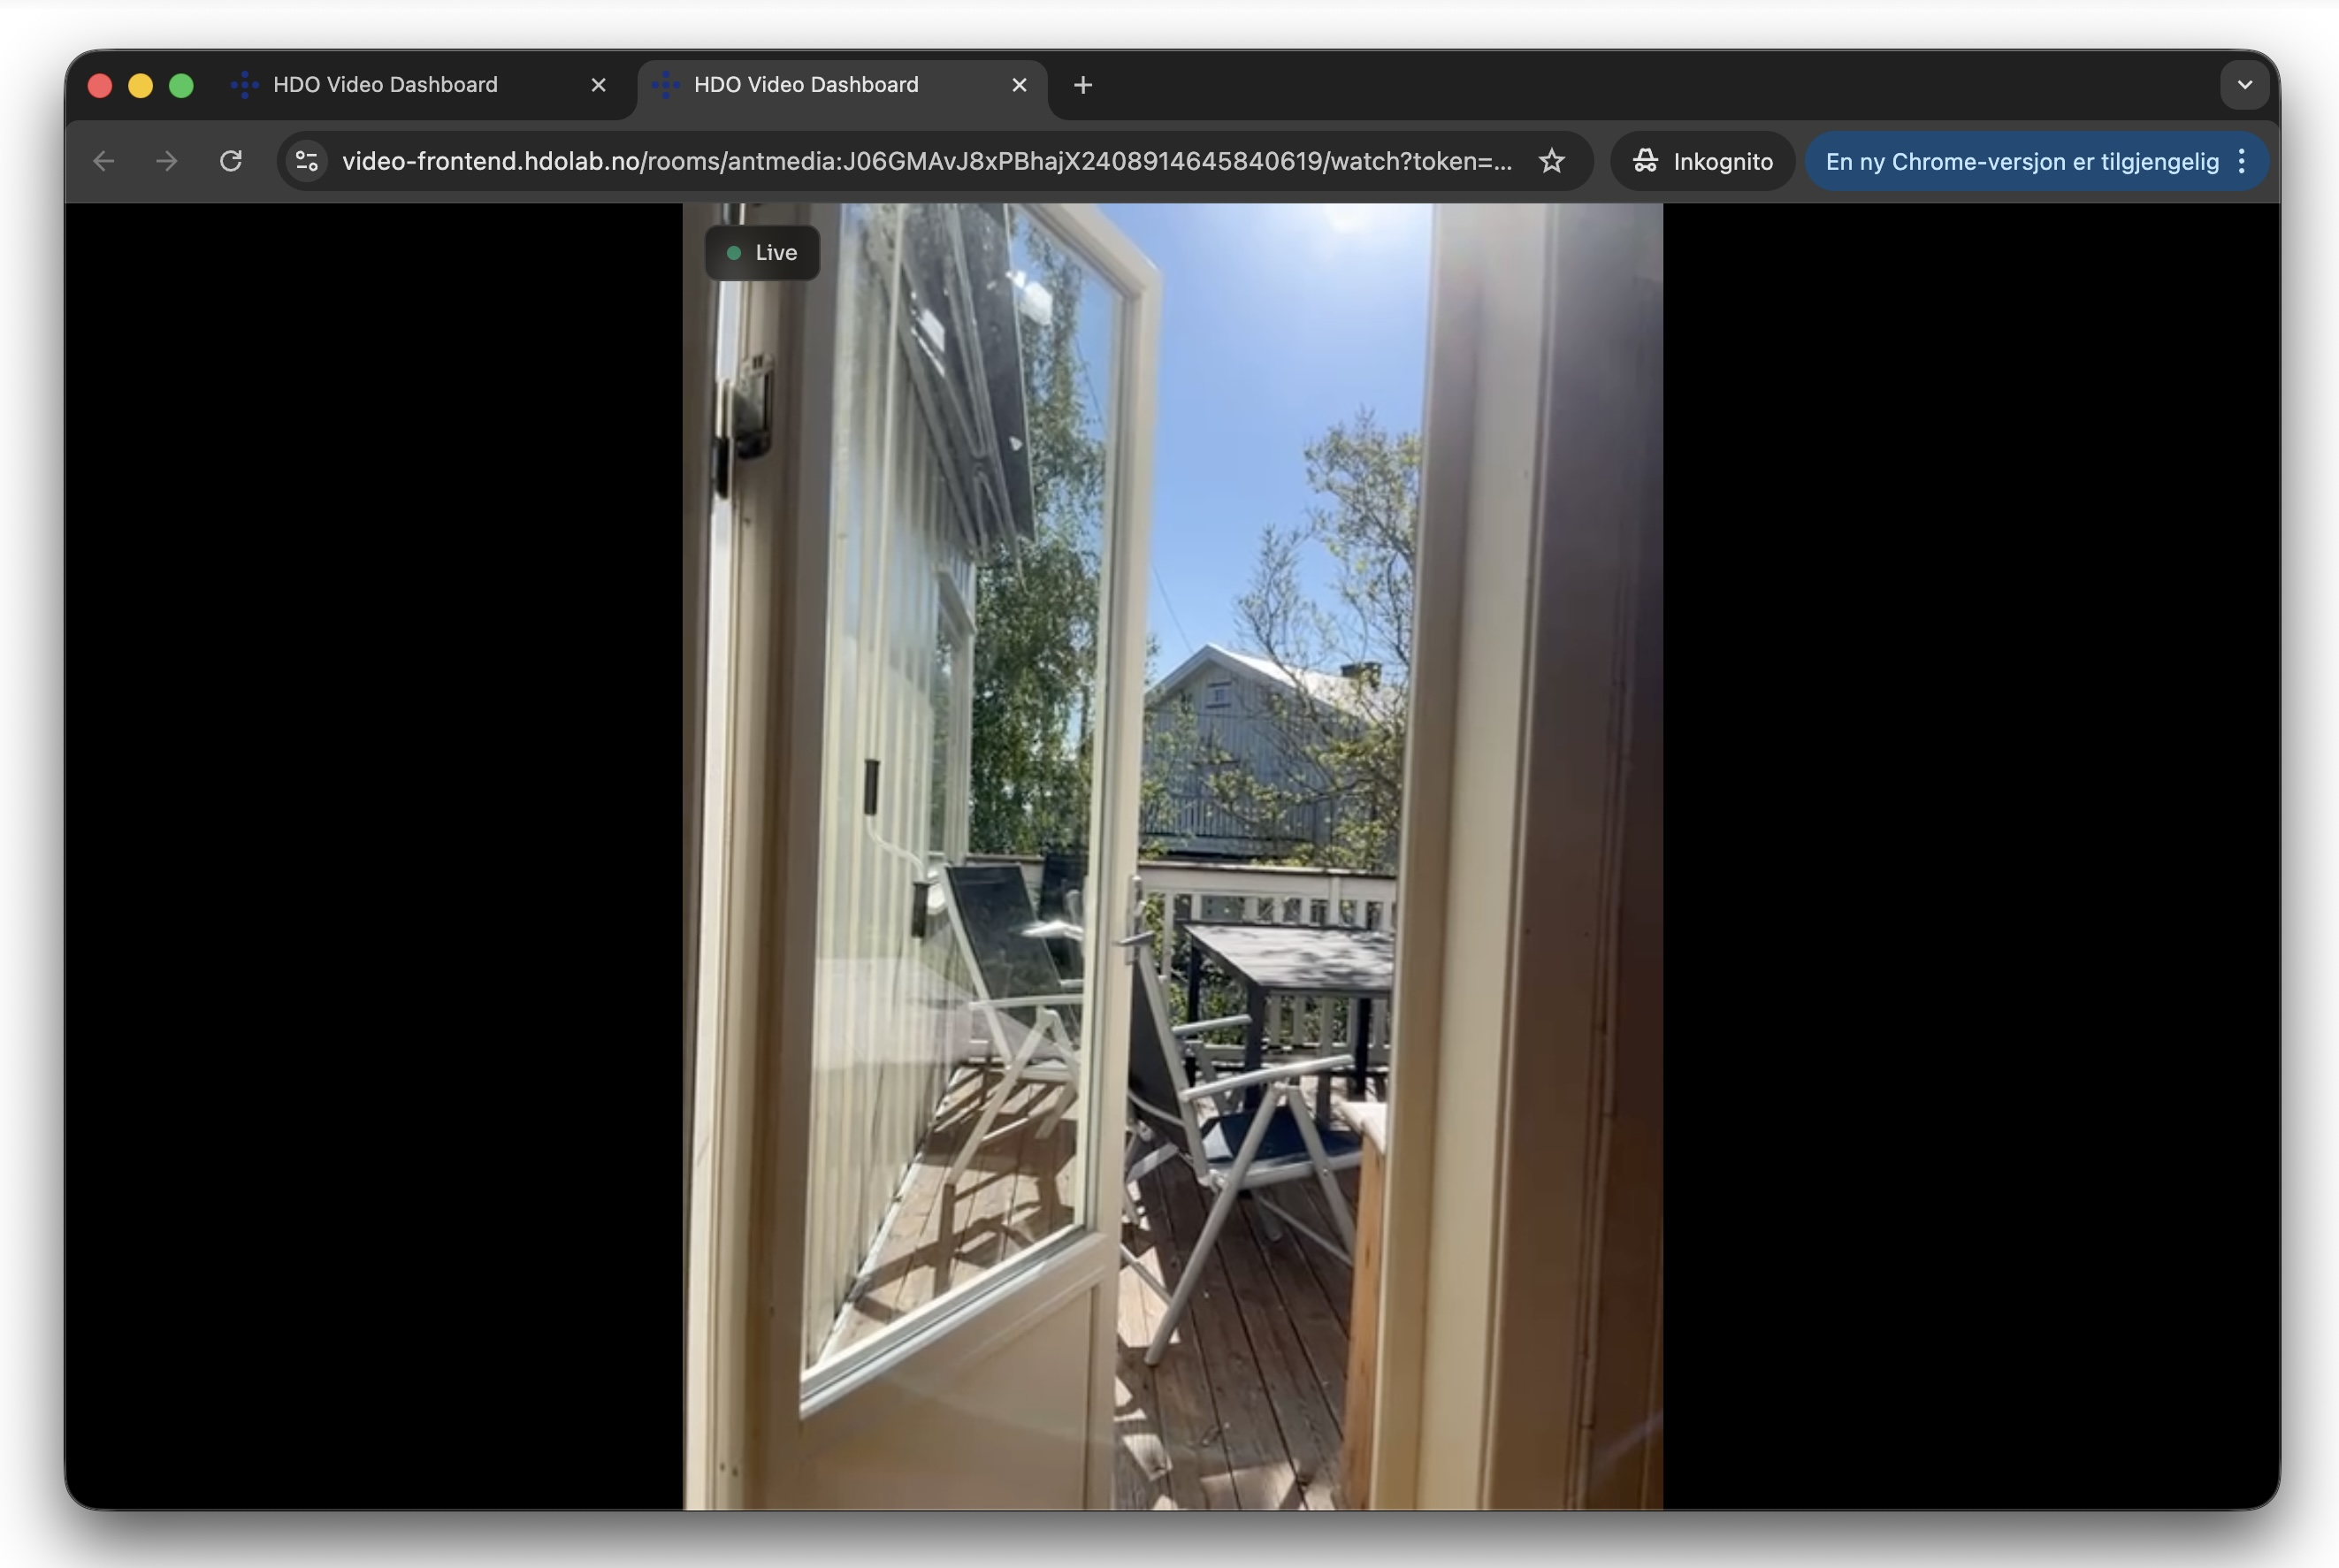
\includegraphics[width=\linewidth]{figures/hdo-watch.jpg}
    \caption*{(b) \texttt{Watch}}
  \end{minipage}
  \caption{Aktiv videostrøm i \texttt{antmedia-rom-1}: avsender (mobil) og mottaker (PC).}
  \label{fig:frontend-broadcast-watch}
\end{figure}

For NHN-rom videresender \texttt{Watch}- og \texttt{Broadcast}-lenkene brukeren direkte til NHNs egen
videotjeneste, og strømmingen foregår derfor utenfor demo-frontenden.

\subsection{Konfigurasjon og distribusjon}
\label{subsec:demo-deploy}

To miljøvariabler styrer tilkoblingen: \texttt{VITE\_API\_BASE\_URL}, som peker på VideoAPI-domenet, og \texttt{VITE\_ANTMEDIA\_BASE\_URL}, som peker på AntMedia Server.
Siden disse bakes inn i JavaScript-bundlen ved bygging må imaget rebygges ved
endring. Dockerfilen bruker et flertrinns-bygg der Node kompilerer applikasjonen, og det endelige trinnet baserer seg på \texttt{nginx:alpine}, som kun serverer det statiske resultatet. Dette gir et lite produksjonsimage uten kjøretidsavhengigheter. HTTPS er påkrevd i praksis, siden moderne nettlesere blokkerer kamera- og mikrofontilgang over ukryptert HTTP.